% CHAPTER 1
\chapter{Introduction}
\label{chp:1_introduction}

\section{Motivation and Problem Definiton}
In recent years, deep neural networks have shown impressive performance in many vision related tasks such as image classification~\cite{he2015deep}, object detection~\cite{redmon2018yolov3} and image segmentation~\cite{long2015fully}. However, they are found to be vulnerable to intentionally crafted small perturbations called adversarial perturbations~\cite{szegedy2013intriguing}. These small perturbations added to the input image successfully change the output of a trained classifier by altering the logits large enough to change its decision to a preferred class~\cite{goodfellow2014explaining}. While these perturbations are optimized in \(\mathcal{L}_p\) spaces~\cite{carlini2017towards}, they are visible to human observers, since small \(\mathcal{L}_p\) does not always correspond to small visible perturbations~\cite{jordan2019quantifying,engstrom2018rotation}.

Multimedia compression standards have been developed to compress visual multimedia such as images and videos to reduce the amount of data with minimum amount of distortion to the perceived output. One of the most fundamental ideas of visual multimedia compression is that human vision is much less sensitive to the information loss in color than the luminance.
%evolution%
This observation is utilized in image compression as a technique known as ``chroma subsampling''. There are variants of chroma subsampling that only subsamples chrominance along horizontal axis (4:2:2) or both horizontal and vertical axes (4:2:0). Without further compression, (4:2:0) chroma subsampling reduces the size of an image effectively to half of its original size. Replacing the chroma components of the pixels in by neighboring chroma components does not yield visible artifacts.
\section{Proposed Methods}
We employ these observations to derive a new type of adversarial attack based on spatial transformations in chroma channels of perceptual colorspaces. We apply spatial transformation only to the chroma components of input image while keeping the luminance component intact. Figure~\ref{fig:flowtochannels} shows the effect of a randomly initialized flow field applied to the luminance, chrominance and both set of channels. It is clear that spatial transformation in luminance channels causes visible distortions while chrominance only spatial transformations cause very subtle changes for human vision. This effect is much more highlighted when only the differences are observed after applying a flow field. Figure \ref{fig:outofgamut} shows the absolute pixel difference from the initial image when the same flow field is applied to RGB, \(C_{b}C_{r}\) and a*b* channels, respectively.
\begin{figure}[t]
    \centering
    \begin{subfigure}[b]{.30\linewidth}
        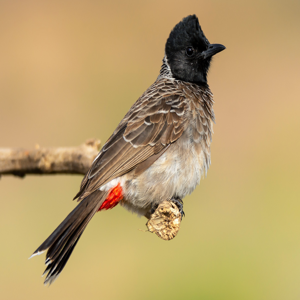
\includegraphics[width=\linewidth]{img.png}
        %        \caption{Original}
        \caption{}
    \end{subfigure}
    \begin{subfigure}[b]{.30\linewidth}
        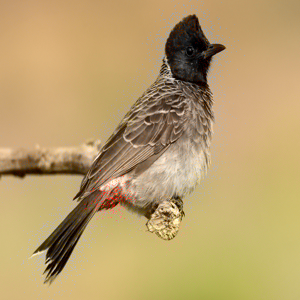
\includegraphics[width=\linewidth]{flowed_cbcr.png}
        %        \caption{Flow to CbCr channels}
        \caption{}
    \end{subfigure}
    \begin{subfigure}[b]{.30\linewidth}
        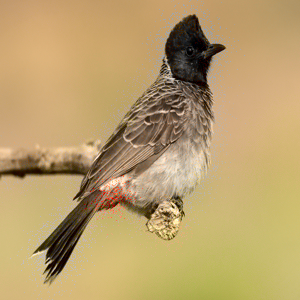
\includegraphics[width=\linewidth]{flowed_ab.png}
        %       \caption{Flow to \(a^*b^*\) channels}
        \caption{}
    \end{subfigure}
    \begin{subfigure}[b]{.30\linewidth}
        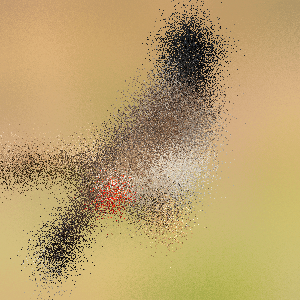
\includegraphics[width=\linewidth]{flowed_rgb.png}
        %      \caption{Flow to RGB channels}
        \caption{}
    \end{subfigure}
    \begin{subfigure}[b]{.30\linewidth}
        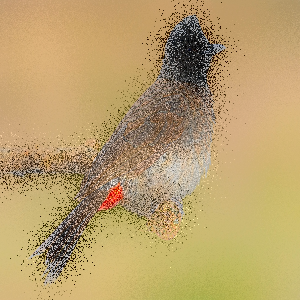
\includegraphics[width=\linewidth]{flowed_y.png}
        %     \caption{Flow to Y channel}
        \caption{}
    \end{subfigure}
    \begin{subfigure}[b]{.30\linewidth}
        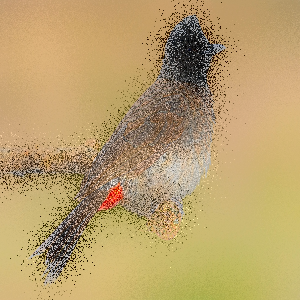
\includegraphics[width=\linewidth]{flowed_l.png}
        %\caption{Flow to L channel}
        \caption{}
    \end{subfigure}
    \caption{Effect of flow field applied to different channels, (a) original image, Images where flow field is applied to (b) \(C_{b}C_{r}\), (c) \(a^*b^*\), (d) RGB, (e) Y and (f) L channel. The magnitude of the flow is scaled up to emphasize the effect for illustration.}\label{fig:flowtochannels}
\end{figure}

\begin{figure}[t]
    \centering
    \begin{subfigure}[b]{.23\linewidth}
        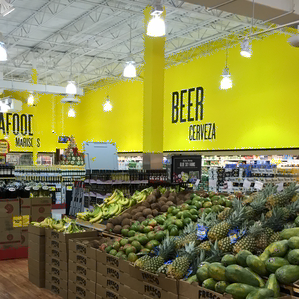
\includegraphics[width=\linewidth]{diff/209_lab_adv.png}
        \caption{}
    \end{subfigure}
    \begin{subfigure}[b]{.23\linewidth}
        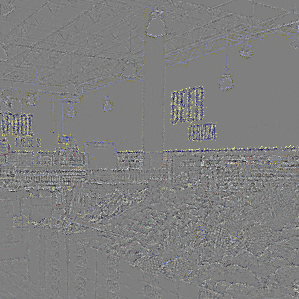
\includegraphics[width=\linewidth]{diff/209_rgb_diff.png}
        \caption{}
    \end{subfigure}
    \begin{subfigure}[b]{.23\linewidth}
        
\includegraphics[width=\linewidth]{diff/209_ycbcr_diff.png}
        \caption{}
    \end{subfigure}
    \begin{subfigure}[b]{.23\linewidth}
        
\includegraphics[width=\linewidth]{diff/209_lab_diff.png}
        \caption{}
    \end{subfigure}
    \caption{Visual difference from flow field applied to different channels, (a) original image, Visualization of pixel differences where flow field is applied to (b) RGB, (c) \(C_{b}C_{r}\), (d) \(a^*b^*\) channels. The magnitude of the flow is scaled up and contrast of the pixel differences is increased to increase the visibility for illustration. }\label{fig:diff}
\end{figure}

\begin{figure*}[t]
    \centering
    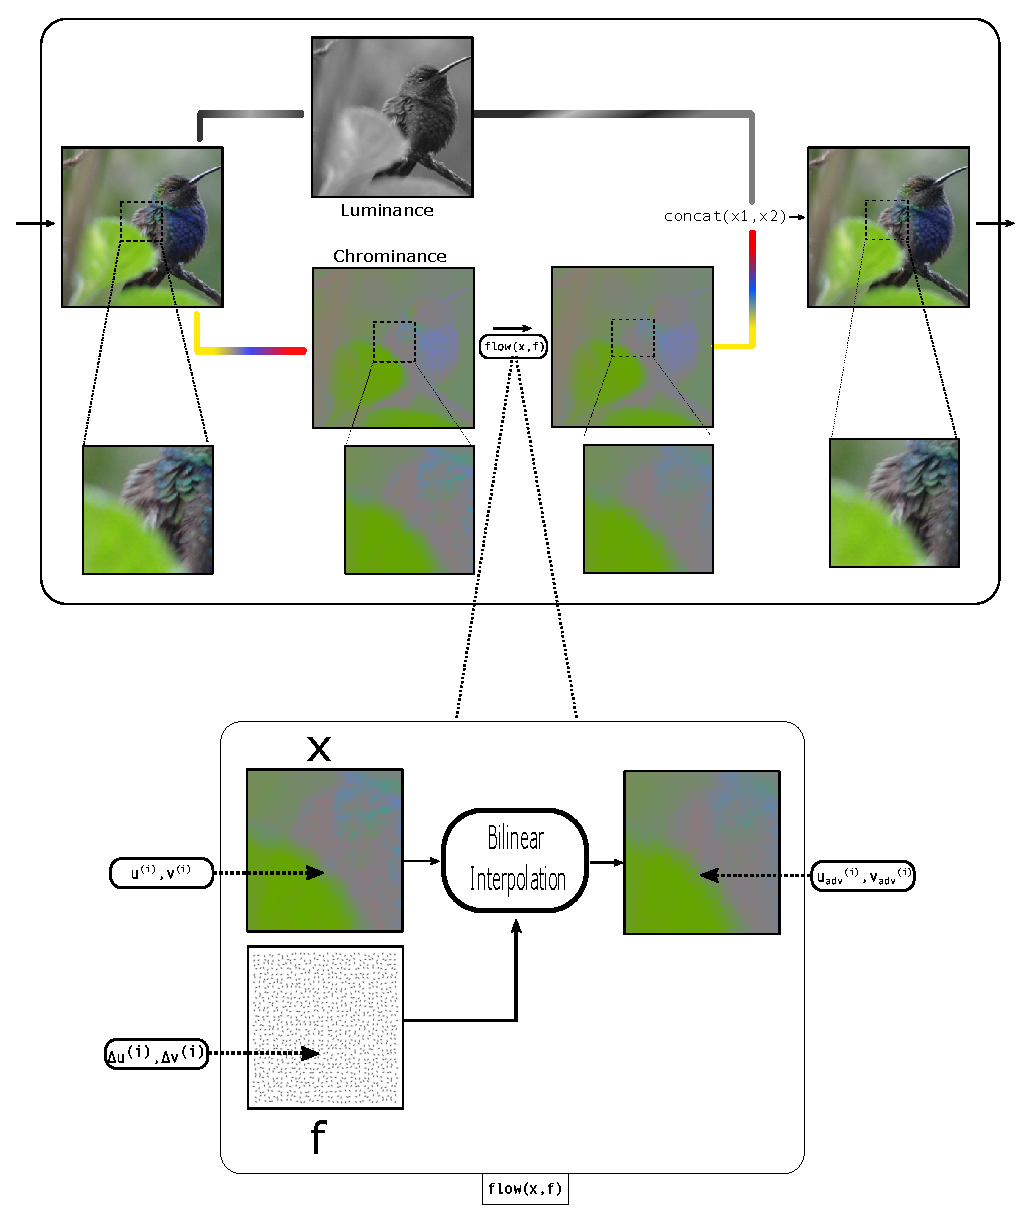
\includegraphics[width=0.8\linewidth]{illustration/drawing.eps}
    \caption{Visual illustration of the proposed adversarial example generation method. Luminance and chrominance channels are Y and \(C_{b}C_{r}\) when \(YC_{b}C_{r}\) colorspace and L and \(a^*b^*\) when CIELAB colorspace is used. Visual representation of flow field, subpixel restriction by \(\tanh\) and conversion of concatenated image back to RGB colorspace is omitted for brevity.}\label{fig:algorithm}
\end{figure*}

\section{Contributions of the Study}

The main findings of this thesis is published in a paper~\cite{aydin2019imperceptible} and the subject is further elaborated in this thesis. The contributions of this work can be summarized as following;
\begin{itemize}
    \item Utilization of the findings of human vision and ideas from multimedia compression to make imperceptible changes on images without any \(L_p\) norm restriction or regularization.
    \item A novel method to generate adversarial examples with little to no perceptual distortion by applying spatial transformations in chroma channels of perceptual colorspaces.
    \item Colorfulness analysis of NIPS2017 Adversarial Challenge dataset.
\end{itemize}

\section{Organization of the Thesis}
This thesis is organized as follows. Chapter \ref{chp:1_introduction} provides an introduction on the thesis topic, explaining the motivation, defines the problem attacked and briefly explains the methods and contributions of the thesis. Chapter \ref{chp:2_literature} mentions the literature about the thesis topic, presents the types and classifications of adversarial attacks and methods for generating imperceptible types of adversarial attacks or methods to improve perceptual quality of adversarial examples. Chapter \ref*{chp:3_methodology} explains the methodology of the method proposed in this thesis in a detailed manner. It starts with spatial transformations, then explains spatially transformed adversarial examples and colorspaces to build the foundation of this thesis. Then, it explains the method proposed in this thesis. Chapter \ref{chp:4_results} mentions the setup of the experiments and presents the experimental results. Chapter \ref{chp:5_discussion} provides a discussion about the results presented in Chapter \ref{chp:5_discussion}, explains the implications of the results and mentions the failure cases, discussing the possible reasons. Chapter \ref{chp:6_conclusion} draws conclusions on the thesis along with possible future studies of the new research questions with the thesis.

